\section{NovelGym}
\label{sec:novelgym}

NovelGym\footnote{The project website and codebase are available at \url{https://github.com/tufts-ai-robotics-group/NovelGym}. Detailed tutorials, PDDL specifications, configuration file formats, and hyperparameter settings are provided in~\citet{goel2024novelgym}.} extends and generalizes the ideas introduced in NovelGridworlds into a flexible ecosystem for developing and benchmarking open-world agents. While NovelGridworlds provides a fixed set of tasks and novelties suitable for initial evaluation, NovelGym introduces a formal framework for defining environments and their transformations, a modular software architecture for rapid development of tasks, novelties, and agent systems, and a comprehensive evaluation protocol with adaptation-focused metrics. The ecosystem supports single-agent and multi-agent scenarios, accommodates symbolic planning agents, reinforcement learning agents, and hybrid architectures, and enables composable novelty injection. The environment representation introduced in \cref{fig:ng_environment} serves as the basis for the formalism presented below.

\subsection{Environment Formalism}
\label{sec:ng_environment}

We formalize the environment as a tuple $E = \langle G, \mathcal{E}, \mathcal{R}, \States, \Actions, \tau, C \rangle$, where each component is defined as follows.

\paragraph{Grid.} $G \subseteq \mathbb{Z}^2$ represents the set of all grid cells in a two-dimensional gridworld. For an $m \times n$ grid, each cell is identified by its position $(i, j)$ with $1 \leq i \leq m$ and $1 \leq j \leq n$.

\paragraph{Entities.} $\mathcal{E} = \{\langle t_1, P_{e_1} \rangle, \langle t_2, P_{e_2} \rangle, \ldots, \langle t_n, P_{e_n} \rangle\}$ is the set of all entities in the environment. Each entity $e = \langle t, P_e \rangle$ consists of a type $t$ drawn from the set of all entity types $T$ and a set of properties $P_e$ drawn from a global property set $P$. Some entities are \emph{dynamic}, meaning they can take actions in the environment and influence state transitions. Entities can be located on grid cells, in an agent's inventory, or nested within other entities.

\paragraph{Recipes.} $\mathcal{R} = \{r_1, r_2, \ldots, r_r\}$ is a set of transformation rules. Each rule $r : \mathcal{E}^* \times L_r \rightarrow \mathcal{E}^*$ defines how one or more entities can be transformed into another set of entities, where $L_r \subseteq G$ restricts the locations at which the recipe can be applied. For example, a recipe might specify that one unit of platinum, one stick, and two planks can be combined at the crafting table to produce a platinum axe.

\paragraph{States, actions, and transitions.} $\States$ is the set of all possible states, capturing the locations and properties of all entities. $\Actions = \{a_1, a_2, \ldots, a_a\}$ is the set of primitive actions. While all actions are syntactically available in every state, some produce effects only in specific contexts. The transition dynamics are defined as:
\[
\tau : \States \times \Actions \times (\Actions_{e_1}, \Actions_{e_2}, \ldots, \Actions_{e_m}) \rightarrow \States,
\]
where the tuple $(\Actions_{e_1}, \ldots, \Actions_{e_m})$ captures the actions taken by dynamic entities in the environment, reflecting the multi-agent nature of the system.

\paragraph{Cost function.} $C : \States \times \Actions \rightarrow \Real^+$ assigns a non-negative cost to each state-action pair. Costs can depend on context; for example, breaking a tree may cost less when the agent holds a tool.

\subsection{Agent Formalism}
\label{sec:ng_agent}

An agent is defined as $\mathcal{A} = \langle Sen, Act, \mathcal{K}, \Pi \rangle$, where $Sen$ denotes the agent's sensors that generate observations $O$ of the world, $Act$ denotes actuators that can affect the world, $\mathcal{K}$ is a knowledge repository that may be initially empty and accumulate knowledge over time, and $\Pi : O \rightarrow \Actions$ maps observations to actions.

Observations can take multiple forms depending on the agent's sensor configuration. NovelGym supports LiDAR-like sensors that return distances to entities at angular increments, image-based local view representations using one-hot vector encodings of entity types on a grid around the agent, and symbolic state descriptions expressed in PDDL. This flexibility allows the same environment to interface with planning agents, reinforcement learning agents, and hybrid systems without modification.

% FIGURE PLACEHOLDER: Sensor representations (LiDAR and local view)
\begin{figure}[t]
    \centering
    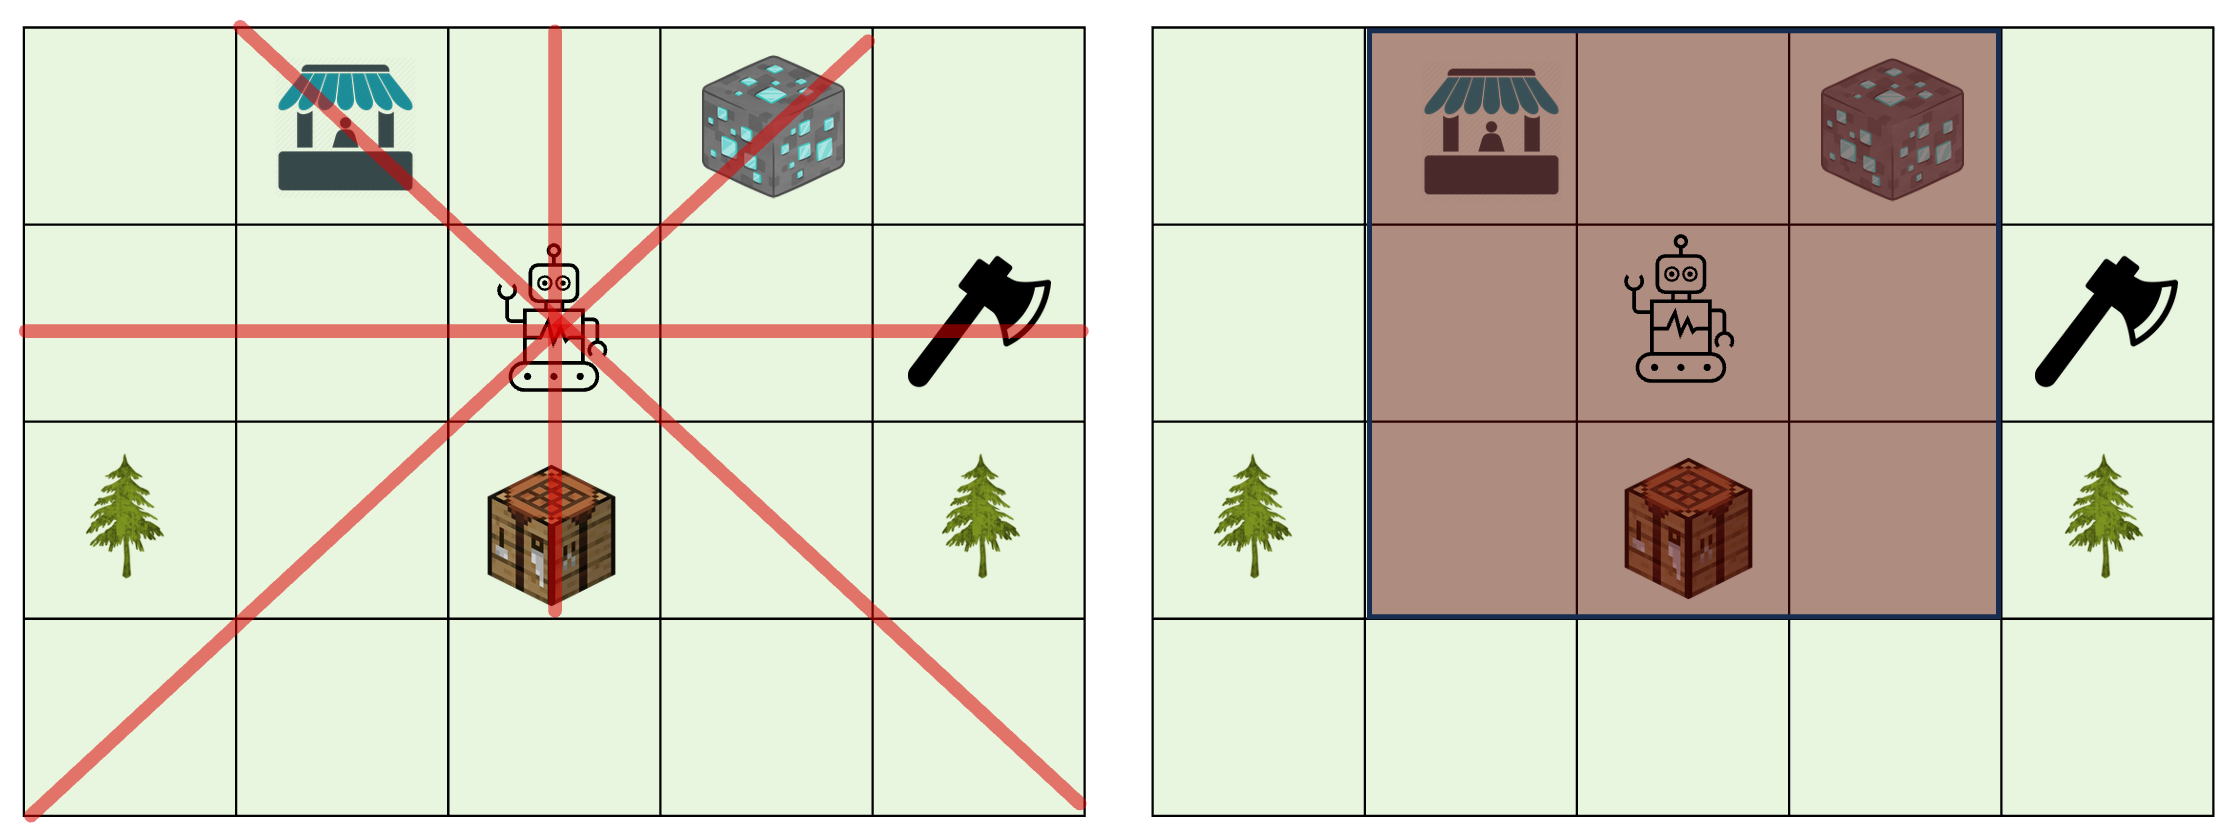
\includegraphics[width=0.7\textwidth]{figures/chapter3/sensor_rep.png}
    \caption{Illustration of the agent's sensor representations in NovelGym. (Left) A LiDAR-like representation emitting beams at angular increments. (Right) An image-based local view representation using one-hot vector encodings.}
    \label{fig:ng_sensors}
\end{figure}

The agent's behavior function $\Pi$ can be implemented using symbolic planning, reinforcement learning, or hybrid approaches, as formalized in \cref{sec:symbolic_planning,sec:rl,sec:hybrid}. Actions can be primitive (e.g., \texttt{move-forward}) or parameterized operators (e.g., \texttt{approach <entity>}) that are executed through sequences of primitive actions by an internal planner.


\subsection{Novelty as Environment Transformation}
\label{sec:ng_novelty}

NovelGym formalizes novelty through the concept of environment transformations. A transformation is a function $\nu : E \rightarrow E'$ that modifies one or more components of the environment. This formalism complements the class-based taxonomy introduced in \cref{sec:ngw_novelty_taxonomy}: while the taxonomy categorizes novelties by which aspect of the agent's model they affect, the transformation formalism specifies precisely which components of the environment are modified and how. Six categories of transformation are supported:
\begin{itemize}[leftmargin=*]
    \item \textbf{Layout changes}: The grid $G$ is modified such that $G \neq G'$, altering the spatial structure of the environment.
    \item \textbf{Entity alterations}: The set of entities $\mathcal{E}$ changes such that $\mathcal{E} \neq \mathcal{E}'$, introducing new entities or modifying existing ones.
    \item \textbf{Recipe modifications}: The transformation rules $\mathcal{R}$ change such that $\mathcal{R} \neq \mathcal{R}'$, altering how items can be crafted.
    \item \textbf{Action alterations}: The action set $\Actions$ changes such that $\Actions \neq \Actions'$, adding, removing, or modifying available actions.
    \item \textbf{Transition dynamics changes}: For some state $s \in \States$ and action $a \in \Actions$, $\tau(s, a) \neq \tau'(s, a)$, changing how the environment responds to the agent's actions.
    \item \textbf{Cost function alterations}: The cost function $C$ changes such that $C \neq C'$, modifying the cost associated with certain actions.
\end{itemize}

Critically, these transformations are \emph{composable}. Multiple transformations can be applied in sequence to construct complex novelty scenarios, enabling the simulation of environments that undergo continual change. Whether a particular transformation constitutes a novelty for a given agent depends on the agent's knowledge, perceptions, and representations. An agent that navigates using LiDAR sensors may be unaffected by a layout transformation that changes the visual appearance of walls, whereas an agent relying on image-based observations would encounter novelty.


\subsection{Architecture and Implementation}
\label{sec:ng_architecture}

The NovelGym ecosystem is composed of two main components: the environment and the agent training architecture. A novelty injector module transforms the environment based on specified configurations.

% FIGURE PLACEHOLDER: NovelGym system architecture diagram (Figure 3 from the paper)
\begin{figure}[t]
    \centering
    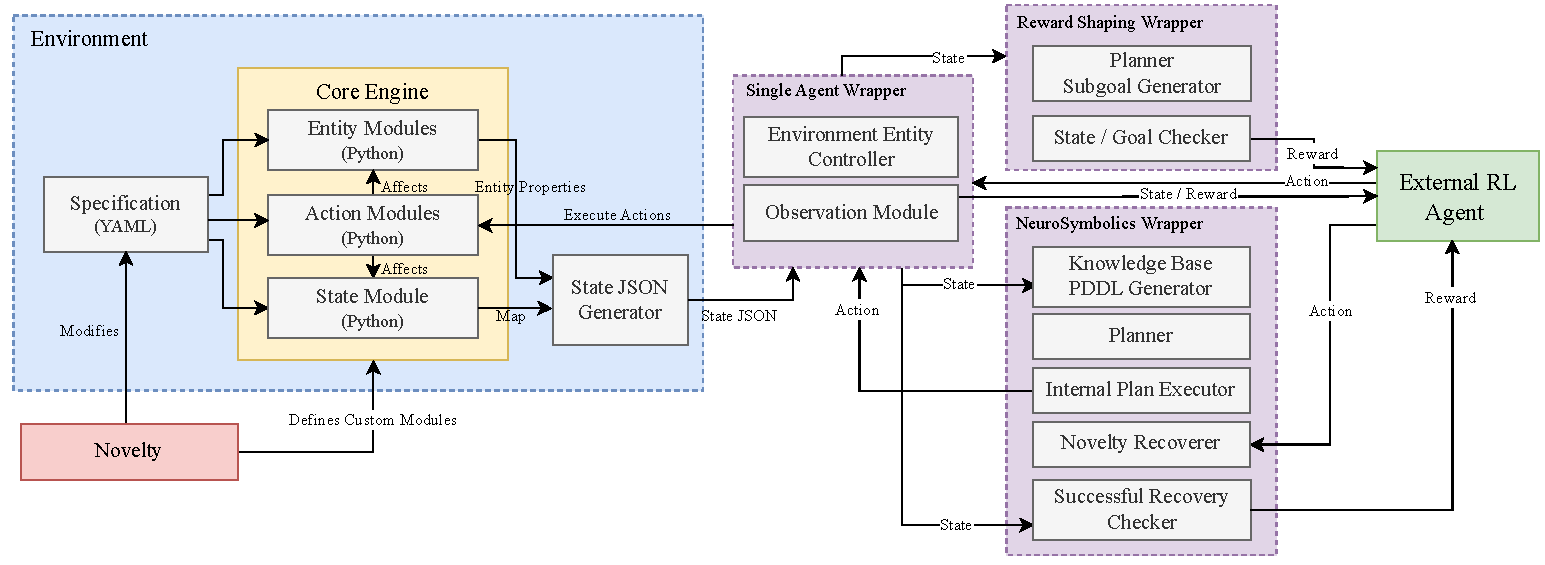
\includegraphics[width=\textwidth]{figures/chapter3/novelgym_architecture.pdf}
    \caption{System design of the NovelGym ecosystem. Blue highlights the environment modules and purple highlights the agent modules. The novelty injector (red) transforms the environment based on specified configurations.}
    \label{fig:ng_architecture}
\end{figure}

\paragraph{Environment.} The environment is implemented on top of PettingZoo~\citep{terry2021pettingzoo} and OpenAI Gym~\citep{brockman2016openai}, supporting multi-agent systems natively. It comprises several modules:
\begin{itemize}[leftmargin=*]
    \item A \emph{specification module} that reads YAML configuration files and initializes the world, including entities, actions, and their properties.
    \item An \emph{entity module} responsible for entity initialization and customization, including configurable properties such as breakability.
    \item An \emph{action module} that implements primitive actions and higher-level operators and ensures the world state is updated upon execution.
    \item A \emph{state module} that maintains the world map, tracks entities, and manages scheduled state updates for durative actions.
    \item A \emph{novelty module} that modifies entity, action, and state modules according to the novelty configuration.
\end{itemize}

\paragraph{Agent training architecture.} The agent-side architecture is designed to support hybrid planning and learning systems through three components:
\begin{itemize}[leftmargin=*]
    \item A \emph{single-agent wrapper} that converts the multi-agent PettingZoo environment into a single-agent interface by controlling all non-primary agents. It includes an observation conversion module that can produce LiDAR, local-view, or symbolic state representations. For object-centric observation spaces, the wrapper automatically expands observation and action spaces when new entities or actions appear due to novelty.
    \item A \emph{neurosymbolic wrapper} that maintains a PDDL-based knowledge base, automatically generates PDDL domain and problem files from the environment configuration, interfaces with a planner (MetricFF~\citep{hoffmann2003metricff}) to generate plans, executes plan operators through a plan executor, and provides a novelty recovery component for implementing adaptation routines.
    \item A \emph{reward-shaping wrapper} that uses the integrated planner to generate subgoals from the symbolic plan and shapes rewards by monitoring whether subgoals are achieved during learning. This wrapper enables sophisticated routines for novelty handling that combine planning and learning.
\end{itemize}

The architecture also integrates a modular reinforcement learning framework (Tianshou~\citep{weng2022tianshou}), enabling users to experiment with various learning algorithms. The modularity of the system played a crucial role in enabling the implementation of complex hybrid agent architectures evaluated in this chapter and developed further in the RapidLearn line of work~\citep{goel2022rapidlearn}.


\subsection{Evaluation Protocol and Metrics}
\label{sec:ng_evaluation}

NovelGym introduces an evaluation protocol consisting of four phases, illustrated in~\cref{fig:ng_metrics}:
\begin{enumerate}[leftmargin=*]
    \item \textbf{Initial training}: The agent is trained in a controlled, novelty-free environment until its knowledge base or policy is sufficient to solve the task.
    \item \textbf{Novelty injection}: A transformation is applied to the environment. The agent's performance is monitored immediately to assess the impact.
    \item \textbf{Adaptation}: The agent interacts with the transformed environment to recalibrate its approach.
    \item \textbf{Post-adaptation evaluation}: After a predefined adaptation period or upon meeting a convergence criterion, the agent's performance is assessed in the novel environment.
\end{enumerate}

\begin{figure}[t]
    \centering
    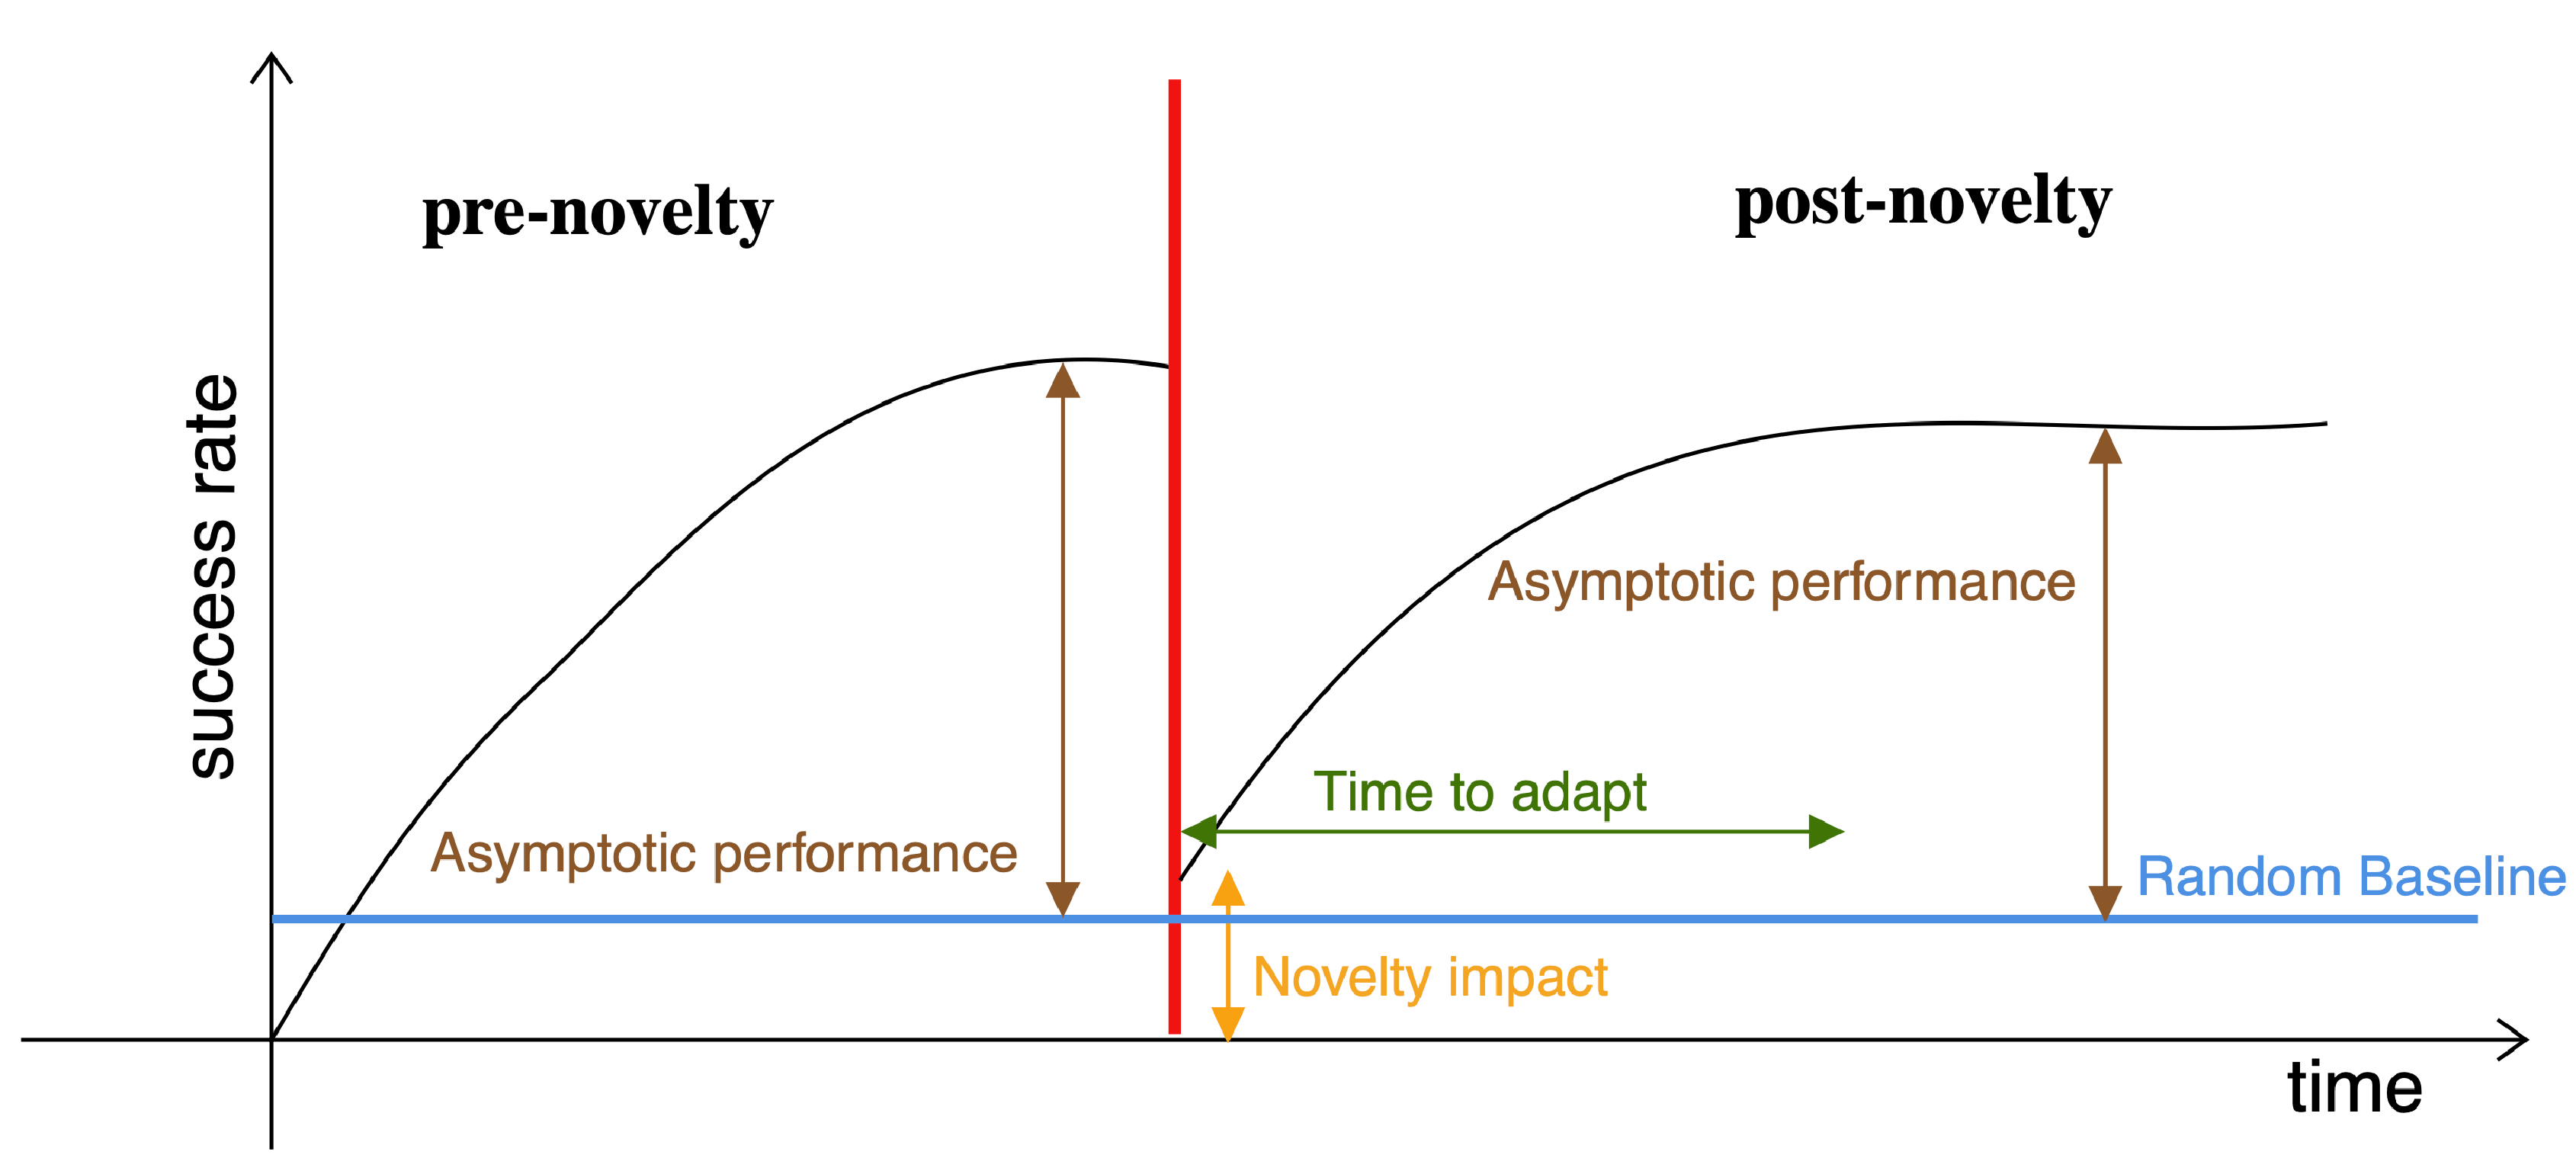
\includegraphics[width=0.85\textwidth,keepaspectratio]{figures/chapter3/eval_metrics.pdf}
    \caption{Illustration of the NovelGym evaluation protocol and performance over time: success rate as training progresses, with novelty injection dividing pre- and post-novelty regimes. The annotated regions correspond to the metrics in \cref{sec:ng_evaluation} (pre-novelty asymptotic performance, novelty impact, adaptation, and post-novelty performance).}
    \label{fig:ng_metrics}
\end{figure}

Five evaluation metrics are defined to capture different aspects of an agent's behavior under novelty:
\begin{enumerate}[leftmargin=*]
    \item \textbf{Pre-novelty asymptotic performance} ($S_\text{pre}$): The agent's success rate after convergence in the pre-novelty task.
    \item \textbf{Novelty impact} ($I_\text{novelty}$): The immediate performance drop upon novelty introduction, defined as $I_\text{novelty} = S_\text{pre} - S_\text{immediate post}$.
    \item \textbf{Time to adapt} ($T_\text{adapt}$): The number of time steps, actions, or wall-clock time required for the agent to reach a convergence criterion after novelty injection.
    \item \textbf{Asymptotic adaptation performance} ($S_\text{post}$): The agent's success rate after adaptation has converged in the post-novelty scenario.
    \item \textbf{Post-adaptation efficiency} ($\Delta t$): The difference in average task completion time before and after novelty, defined as $\Delta t = t_\text{pre} - t_\text{post}$. A positive value indicates that the novelty ultimately allowed the agent to find a more efficient solution.
\end{enumerate}

These metrics extend the M1, M2, and M3 metrics of NovelGridworlds by explicitly capturing adaptation dynamics. While the earlier metrics focus on cost and detection, the NovelGym metrics additionally measure the speed of adaptation, the severity of the initial performance drop, and whether the agent can exploit beneficial novelties.


\subsection{Benchmark Task and Novelties}
\label{sec:ng_task}

The benchmark task in NovelGym is a Minecraft-inspired pogostick crafting task. The agent operates in a two-room gridworld environment containing resources (oak trees, diamond ore, platinum blocks), a crafting table, and a trader (see \cref{fig:ng_environment}). The agent must collect resources, craft intermediary items, trade with the trader, and ultimately craft a pogostick. A simplified version of the task was used to make it tractable for reinforcement learning agents while preserving the sequential, multi-step nature of the crafting challenge.

Five environment transformations were selected for evaluation, spanning detrimental and beneficial categories:
\begin{enumerate}[leftmargin=*]
    \item \textbf{Axe} (detrimental): Trees become unbreakable unless the agent uses a newly introduced axe item.
    \item \textbf{Chest} (beneficial): A chest containing all ingredients for crafting a pogostick is placed in the environment, along with a new action to approach it.
    \item \textbf{Trader} (detrimental): The agent must maintain one grid cell of distance from the trader for the trade action to succeed.
    \item \textbf{Fence} (detrimental): All oak logs are surrounded by breakable fences that must be removed before the logs can be accessed.
    \item \textbf{Fire} (detrimental): The crafting table is set on fire, and the agent must collect a water bucket and extinguish the fire before crafting.
\end{enumerate}

% FIGURE PLACEHOLDER: Pre-novelty and post-novelty environment illustrations (Figure 5 from the paper)
\begin{figure}[t]
    \centering
    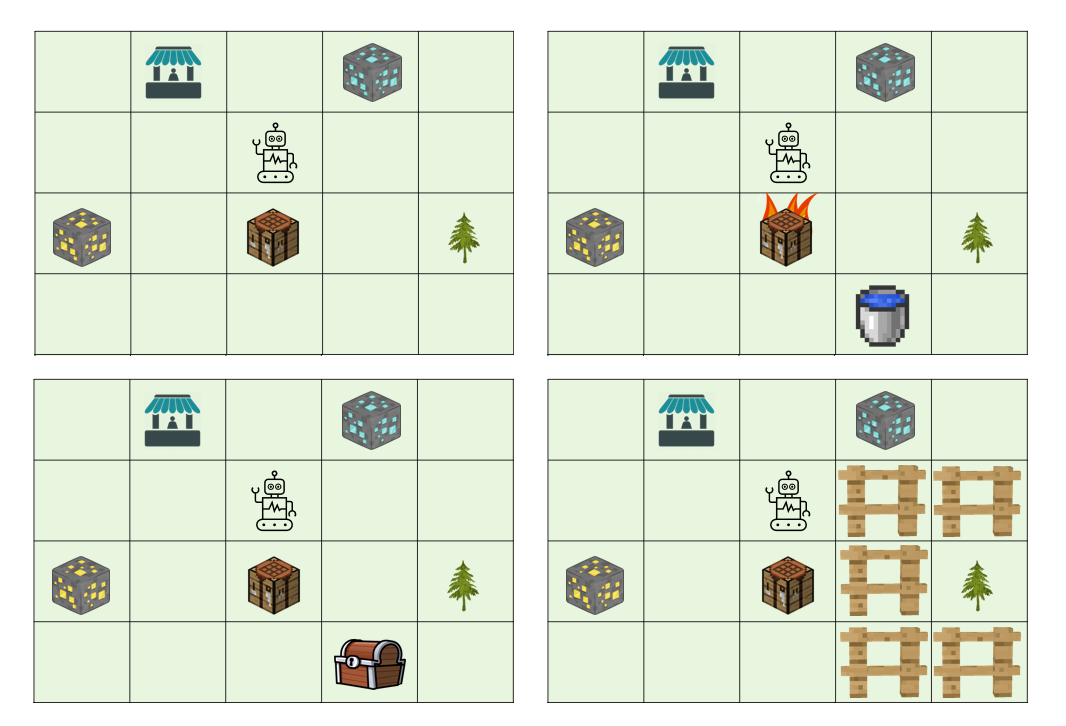
\includegraphics[width=\textwidth]{figures/chapter3/novelties.png}
    \caption{Illustration of the pre-novelty environment and three novelty scenarios: fire, fence, and chest. Each transformation modifies specific components of the environment formalism.}
    \label{fig:ng_novelties}
\end{figure}

Twelve transformations are implemented in total, including additional novelties such as \emph{busy traders}, \emph{moving traders}, \emph{multi-room layouts}, and \emph{portal treasure}\footnote{A complete list of all implemented transformations and their specifications is provided in~\citet{goel2024novelgym}.}.


\subsection{Agent Architectures}
\label{sec:ng_agents}

Four agent architectures were benchmarked, spanning hybrid and transfer learning approaches:
\begin{itemize}[leftmargin=*]
    \item \textbf{RapidLearn$^+$ (PPO+ICM)}: A hybrid planning and learning architecture that uses symbolic planning for the pre-novelty task and instantiates a reinforcement learning problem when plan execution fails due to novelty. The RL component uses PPO~\citep{schulman2017proximal} augmented with the Intrinsic Curiosity Module (ICM)~\citep{pathak2017curiosity} for exploration. This architecture is a direct implementation of the method introduced in~\citet{goel2022rapidlearn}.
    \item \textbf{RapidLearn (PPO)}: The same hybrid architecture without ICM.
    \item \textbf{Transfer RL (PPO)+ICM}: A pure reinforcement learning approach that pre-trains on the base task and transfers weights to the post-novelty task, with automatic expansion of observation and action spaces, augmented with ICM.
    \item \textbf{Transfer RL (PPO)}: The same transfer approach without ICM.
\end{itemize}

All agents used a LiDAR-like observation space with beams emitted at $\frac{\pi}{4}$ increments for each entity type, producing an observation vector of size $8 \times |\mathcal{E}|$, augmented by inventory and selected-item sensors. The symbolic description for hybrid agents was represented in PDDL with a type hierarchy, predicates for entity relations, and operators defined with preconditions and effects.


\subsection{Experimental Results}
\label{sec:ng_results}

All agents achieved perfect pre-novelty performance ($S_\text{pre} = 1.0$), with the RL agents requiring 4 million training time steps to reach this level. Results are organized across two tables. \Cref{tab:ng_performance} reports performance metrics---pre-novelty success rate, novelty impact, and post-adaptation success rate---which capture how severely each novelty degrades the agent and whether the agent ultimately recovers. \Cref{tab:ng_efficiency} reports efficiency metrics---adaptation time and post-adaptation efficiency---which capture how quickly the agent adapts and whether the adapted strategy is more or less costly than the original. Together, these tables provide a comprehensive picture of agent behavior under novelty; see~\citet{goel2024novelgym} for additional results and analysis\footnote{All results are averaged across 10 random seeds. A convergence criterion based on success rate and reward thresholds was used to determine when adaptation was complete; see~\citet{goel2024novelgym} for the precise convergence criteria and hyperparameter settings.}. The hybrid agents (RapidLearn and RapidLearn$^+$) are instances of the planning-learning architecture that is formalized and extended in \cref{ch:rapid_learn}.

% TABLE 1: Performance metrics
\begin{table}[t]
\footnotesize
\centering
\begin{tabular}{l l c c c}
\toprule
Novelty & Agent & $S_{\text{pre}} \uparrow$ & $I_{\text{nov}} \downarrow$ & $S_{\text{post}} \uparrow$ \\
\midrule

\textbf{Axe} & RapidLearn$^{+}$(PPO+ICM) & 1 $\pm$ 0 & 0.83 $\pm$ 0.205 & 1.0 $\pm$ 0.0 \\
             & RapidLearn (PPO)          & 1 $\pm$ 0 & 0.69 $\pm$ 0.207 & 1.0 $\pm$ 0.0 \\
             & Transfer RL (PPO)+ICM     & 1 $\pm$ 0 & 1.0 $\pm$ 0.0   & 0.97 $\pm$ 0.021 \\
             & Transfer RL (PPO)         & 1 $\pm$ 0 & 1.0 $\pm$ 0.0   & 0.97 $\pm$ 0.018 \\

\midrule
\textbf{Chest} & RapidLearn$^{+}$(PPO+ICM) & 1 $\pm$ 0 & -- & -- \\
               & RapidLearn (PPO)          & 1 $\pm$ 0 & -- & -- \\
               & Transfer RL (PPO)+ICM     & 1 $\pm$ 0 & 0.0 $\pm$ 0.004 & 1.0 $\pm$ 0.0 \\
               & Transfer RL (PPO)         & 1 $\pm$ 0 & 0.01 $\pm$ 0.009 & 0.98 $\pm$ 0.011 \\

\midrule
\textbf{Trader} & RapidLearn$^{+}$(PPO+ICM) & 1 $\pm$ 0 & 0.45 $\pm$ 0.069 & 0.95 $\pm$ 0.017 \\
                & RapidLearn (PPO)          & 1 $\pm$ 0 & 0.5 $\pm$ 0.07   & 0.96 $\pm$ 0.02 \\
                & Transfer RL (PPO)+ICM     & 1 $\pm$ 0 & 0.96 $\pm$ 0.108 & 0.99 $\pm$ 0.011 \\
                & Transfer RL (PPO)         & 1 $\pm$ 0 & 0.94 $\pm$ 0.128 & 0.96 $\pm$ 0.025 \\

\midrule
\textbf{Fence} & RapidLearn$^{+}$(PPO+ICM) & 1 $\pm$ 0 & 0.38 $\pm$ 0.102 & 0.96 $\pm$ 0.02 \\
               & RapidLearn (PPO)          & 1 $\pm$ 0 & 0.41 $\pm$ 0.052 & 0.95 $\pm$ 0.008 \\
               & Transfer RL (PPO)+ICM     & 1 $\pm$ 0 & 1.0 $\pm$ 0.0   & 0.93 $\pm$ 0.02 \\
               & Transfer RL (PPO)         & 1 $\pm$ 0 & 1.0 $\pm$ 0.0   & 0.92 $\pm$ 0.024 \\

\midrule
\textbf{Fire} & RapidLearn$^{+}$(PPO+ICM) & 1 $\pm$ 0 & 1.0 $\pm$ 0.0   & 0.95 $\pm$ 0.02 \\
              & RapidLearn (PPO)          & 1 $\pm$ 0 & 1.0 $\pm$ 0.0   & 0.95 $\pm$ 0.016 \\
              & Transfer RL (PPO)+ICM     & 1 $\pm$ 0 & 1.0 $\pm$ 0.0   & 0.94 $\pm$ 0.016 \\
              & Transfer RL (PPO)         & 1 $\pm$ 0 & 1.0 $\pm$ 0.0   & 0.96 $\pm$ 0.029 \\

\bottomrule
\end{tabular}
\caption{Performance metrics across novelty scenarios. $S_\text{pre}$: pre-novelty success rate; $I_\text{nov}$: novelty impact (immediate performance drop); $S_\text{post}$: post-adaptation success rate. $\uparrow$ indicates higher is better, $\downarrow$ lower is better. -- indicates the novelty was not detected by the agent. All values are mean $\pm$ standard deviation over 10 seeds.}
\label{tab:ng_performance}
\end{table}


\begin{table}[t]
\footnotesize
\centering
\begin{tabular}{l l c c}
\toprule
Novelty & Agent & $T_{\text{adapt}} \downarrow$ & $\Delta t \downarrow$ \\
\midrule

\textbf{Axe} & RapidLearn$^{+}$(PPO+ICM) & 71040 $\pm$ 17413 & 122.7 $\pm$ 15.61 \\
             & RapidLearn (PPO)          & 68160 $\pm$ 17934 & 116.9 $\pm$ 9.88 \\
             & Transfer RL (PPO)+ICM     & 169440 $\pm$ 97949 & 61.0 $\pm$ 8.95 \\
             & Transfer RL (PPO)         & 114240 $\pm$ 19651 & 63.1 $\pm$ 8.17 \\

\midrule
\textbf{Chest} & RapidLearn$^{+}$(PPO+ICM) & -- & -- \\
               & RapidLearn (PPO)          & -- & -- \\
               & Transfer RL (PPO)+ICM     & 24000 $\pm$ 0 & -3.0 $\pm$ 0.78 \\
               & Transfer RL (PPO)         & 24000 $\pm$ 0 & -3.5 $\pm$ 3.13 \\

\midrule
\textbf{Trader} & RapidLearn$^{+}$(PPO+ICM) & 102720 $\pm$ 20724 & 126.9 $\pm$ 9.97 \\
                & RapidLearn (PPO)          & 96480 $\pm$ 21191 & 122.8 $\pm$ 8.93 \\
                & Transfer RL (PPO)+ICM     & 227040 $\pm$ 112120 & 93.6 $\pm$ 12.05 \\
                & Transfer RL (PPO)         & 350880 $\pm$ 237039 & 89.3 $\pm$ 7.87 \\

\midrule
\textbf{Fence} & RapidLearn$^{+}$(PPO+ICM) & 69120 $\pm$ 15657 & 161.6 $\pm$ 7.6 \\
               & RapidLearn (PPO)          & 66400 $\pm$ 20999 & 168.7 $\pm$ 6.15 \\
               & Transfer RL (PPO)+ICM     & 854400 $\pm$ 52974 & 73.4 $\pm$ 4.7 \\
               & Transfer RL (PPO)         & 701760 $\pm$ 100589 & 90.9 $\pm$ 9.49 \\

\midrule
\textbf{Fire} & RapidLearn$^{+}$(PPO+ICM) & 263520 $\pm$ 81979 & 133.2 $\pm$ 21.38 \\
              & RapidLearn (PPO)          & 252000 $\pm$ 49663 & 142.5 $\pm$ 13.71 \\
              & Transfer RL (PPO)+ICM     & 372960 $\pm$ 198096 & 105.3 $\pm$ 9.85 \\
              & Transfer RL (PPO)         & 127200 $\pm$ 37932 & 103.3 $\pm$ 13.22 \\

\bottomrule
\end{tabular}
\caption{Efficiency metrics across novelty scenarios. $T_\text{adapt}$: time steps required for adaptation to converge; $\Delta t$: difference in task completion time before and after novelty (negative values indicate the agent found a more efficient post-novelty strategy). $\downarrow$ indicates lower is better. All values are mean $\pm$ standard deviation over 10 seeds.}
\label{tab:ng_efficiency}
\end{table}
% 
\paragraph{Novelty impact.} As shown in \cref{tab:ng_performance}, upon novelty injection all agents experienced performance degradation for detrimental novelties, with the fire novelty producing the most severe impact ($I_\text{novelty} = 1.0$ for all agents). Transfer RL agents were generally more sensitive to novelty than hybrid agents, as reflected in higher $I_\text{novelty}$ values. However, hybrid agents showed lower immediate impact in some cases due to their targeted adaptation approach, which activates only upon execution failure.

\paragraph{Adaptation speed.} \Cref{tab:ng_efficiency} reveals that hybrid agents consistently outperformed transfer learning methods on the $T_\text{adapt}$ metric across all novelties. For the fence novelty, hybrid agents adapted in approximately 67{,}000--71{,}000 time steps, while transfer RL agents required 700{,}000--854{,}000 time steps---an order of magnitude difference. This advantage arises from the hybrid architecture's ability to focus learning on the specific subproblem caused by the novelty rather than relearning the entire task.

\paragraph{Post-adaptation performance.} Returning to \cref{tab:ng_performance}, all agents achieved high post-adaptation success rates ($S_\text{post} \geq 0.92$), though none reached perfect scores due to the use of a convergence criterion rather than exhaustive training.

\paragraph{Post-adaptation efficiency and exploiting beneficial novelty.} The post-adaptation efficiency metric $\Delta t$ (\cref{tab:ng_efficiency}) captures an aspect of agent behavior that success rate alone cannot: whether the agent's post-novelty strategy is more or less efficient than its original approach. For detrimental novelties, positive $\Delta t$ values are expected, since the agent must perform additional actions to overcome the novelty (e.g., breaking fences before accessing logs, or extinguishing a fire before crafting). However, the magnitude of $\Delta t$ reveals how much overhead the novelty imposes even after adaptation. For instance, the fence novelty produces large $\Delta t$ values for hybrid agents ($161.6 \pm 7.6$ and $168.7 \pm 6.15$), reflecting the substantial additional navigation and breaking actions required, whereas transfer RL agents achieve lower $\Delta t$ ($73.4 \pm 4.7$ and $90.9 \pm 9.49$), suggesting they discover more efficient post-novelty strategies despite their slower adaptation.

The most notable result appears in the chest novelty, where transfer RL agents achieve \emph{negative} $\Delta t$ values ($-3.0 \pm 0.78$ with ICM and $-3.5 \pm 3.13$ without). A negative $\Delta t$ means the agent completes the task faster after the novelty than before it---the agent has discovered and exploited the shortcut provided by the chest, which bypasses the full crafting chain. This result validates $\Delta t$ as a metric that captures not only degradation but also opportunistic improvement: a well-adapted agent should be able to exploit beneficial novelties, not merely survive detrimental ones. Hybrid agents, by contrast, show no entry for the chest novelty because their plan-monitoring mechanism was never triggered---the original plan continued to succeed, so the chest was never discovered. This highlights a fundamental limitation of failure-driven adaptation: if a novelty does not cause a failure, it remains invisible to the agent, even when exploiting it would substantially improve performance.

\paragraph{Role of curiosity-driven exploration.} The Intrinsic Curiosity Module (ICM) augments the reward signal with a prediction-error-based intrinsic reward, encouraging the agent to visit states where its learned forward model produces high prediction error. The effect of ICM on adaptation is nuanced and novelty-dependent, as reflected in the $\Delta t$ and $T_\text{adapt}$ metrics.

For novelties that require discovering genuinely new states or action sequences, ICM provides a clear benefit. In the fence novelty, Transfer RL with ICM adapts faster ($854{,}400$ vs.\ $701{,}760$ time steps) and achieves lower $\Delta t$ ($73.4$ vs.\ $90.9$), consistent with the hypothesis that curiosity-driven exploration helps the agent discover the fence-breaking strategy. However, for the fire novelty, ICM \emph{increases} adaptation time ($372{,}960$ vs.\ $127{,}200$) and slightly increases $\Delta t$ ($105.3$ vs.\ $103.3$). A plausible explanation is that the fire novelty introduces multiple novel state transitions---the burning crafting table, the water bucket, the extinguish action---all of which generate high prediction error in the forward model. The intrinsic reward thus disperses the agent's exploration across many novel but not equally useful transitions, rather than focusing it on the specific sequence (collect water, extinguish fire, then craft) needed for recovery. In effect, the forward model's prediction error is high in many irrelevant states, providing a noisy exploration signal that interferes with goal-directed adaptation.

For hybrid agents, the effect of ICM is more muted because the planning component constrains the learning problem to a specific subgoal. The RL component operates within a focused subspace defined by the failed operator, limiting the scope over which curiosity-driven exploration can either help or hinder. This further supports the architectural advantage of hybrid systems: by decomposing the adaptation problem, they reduce sensitivity to the quality of the exploration signal.